\uuid{8LgL}
\exo7id{5205}
\titre{exo7 5205}
\auteur{rouget}
\organisation{exo7}
\datecreate{2010-06-30}
\isIndication{false}
\isCorrection{true}
\chapitre{Courbes planes}
\sousChapitre{Coordonnées polaires}
\module{Géométrie}
\niveau{L2}
\difficulte{}

\contenu{
\texte{
Construire l'ensemble des points $M$ de coordonnées polaires $(r,\theta)\in\Rr^2$ vérifiant 

$r=\frac{1}{\sqrt{1+\sin(2\theta)}+\sqrt{1-\sin(2\theta)}}$ (commencer par étudier toutes les symétries de l'ensemble considéré).
}
\reponse{
Notons $\mathcal{E}$ l'ensemble cherché.

Tout d'abord, pour tout réel $\theta$, $1+\sin(2\theta)\geq0$, $1-\sin(2\theta)\geq0$ puis $\sqrt{1+\sin(2\theta)}+\sqrt{1-\sin(2\theta)}>0$, car $\sin(2\theta)$ ne peut valoir simultanément $1$ et $-1$. La fonction $r\mapsto r(\theta)$ est donc définie sur $\Rr$, clairement $2\pi$-périodique.

Ainsi, 

$$M(\theta+2\pi)=[r(\theta+2\pi),\theta+2\pi]=[r(\theta),\theta+2\pi]=M(\theta).$$

On obtient donc l'ensemble complet quand $\theta$ décrit un intervalle de longueur $2\pi$ comme $[-\pi,\pi]$ par exemple.

La fonction $r\mapsto r(\theta)$ est plus paire. Par suite,

$$M(-\theta)=[r(-\theta),-\theta]=[r(\theta),-\theta]=s_{(Ox)}(M(\theta)).$$

On construit l'ensemble des points correspondant à $\theta\in[0,\pi]$ et on obtient l'ensemble complet par symétrie orthogonale d'axe $(Ox)$.

Pour $\theta\in[0,\pi]$, on a clairement $r(\pi-\theta)=r(\theta)$. Par suite,

$$M(\pi-\theta)=[r(\pi-\theta),\pi-\theta]=[r(\theta),\pi-\theta]=s_{(Oy)}(M(\theta)).$$

On construit l'ensemble des points correspondant à $\theta\in[0,\frac{\pi}{2}]$ et on obtient l'ensemble complet par symétrie orthogonale d'axe $(Oy)$ puis par symétrie orthogonale d'axe $(Ox)$.

Pour $\theta\in[0,\frac{\pi}{2}]$, on a clairement $r(\frac{\pi}{2}-\theta)=r(\theta)$. Par suite, en notant $(\Delta)$ la droite d'équation $y=x$,

$$M(\frac{\pi}{2}-\theta)=[r(\frac{\pi}{2}-\theta),\frac{\pi}{2}-\theta]=[r(\theta),\frac{\pi}{2}-\theta]
=s_{(\Delta)}(M(\theta)).$$

On construit l'ensemble des points correspondant à $\theta\in[0,\frac{\pi}{4}]$ et on obtient l'ensemble complet par symétrie orthogonale d'axe $(\Delta)$ puis par symétrie orthogonale d'axe $(Oy)$ et enfin par symétrie orthogonale d'axe $(Ox)$.

Maintenant, pour $\theta\in[0,\frac{\pi}{4}]$,

\begin{align*}
\frac{1}{\sqrt{1+\sin(2\theta)}+\sqrt{1-\sin(2\theta)}}&=
\frac{1}{\sqrt{1+\cos(\frac{\pi}{2}-2\theta)}+\sqrt{1-\cos(\frac{\pi}{2}-2\theta)}}\\
 &=\frac{1}{\sqrt{2\cos^2(\frac{\pi}{4}-\theta)}+\sqrt{2\sin^2(\frac{\pi}{4}-\theta)}}
 =\frac{1}{\sqrt{2}\cos(\frac{\pi}{4}-\theta)+\sqrt{2}\sin(\frac{\pi}{4}-\theta)}\\
 &=\frac{1}{2\cos(\frac{\pi}{4}-(\frac{\pi}{4}-\theta))}=\frac{1}{2\cos\theta}.
\end{align*}

En notant $x$ et $y$ les coordonnées d'un point $M$, on a alors 

$$M\in\mathcal{E}\Leftrightarrow r=\frac{1}{2\cos\theta}\Leftrightarrow r\cos(\theta)=\frac{1}{2}\Leftrightarrow x=\frac{1}{2}.$$

D'où le graphique~:

$$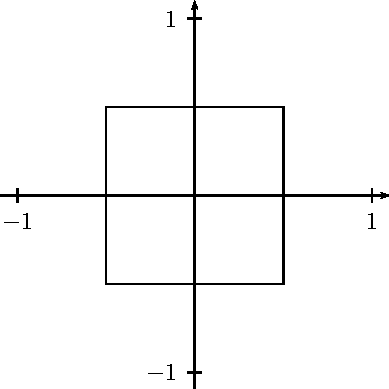
\includegraphics{../images/pdf/8LgL-1.pdf}$$
}
}
